\subsection{Suppressing quantum errors by scaling a surface code logical qubit}

Scaling of the surface code is essential to building large-scale quantum computers. Google Quantum AI has demonstrated successful implementation of the scaling of surface code, showing that increasing the number of qubits can indeed improve the performance of a logical qubit, suppressing the error rate while also dealing with additional problems associated with scaling.

The research team of Google Quantum AI implemented a distance-5 surface code using 72 qubits. By comparing it to a smaller distance-3 code, they observed a reduction in logical error rates per cycle, from 3.028\% to 2.914\%.

This work shows that quantum error correction improves with scaling, essential for developing large quantum systems for applications in cryptography, optimization, and simulations beyond classical capabilities. Using a 72-qubit device, the team showed that larger codes can outperform smaller ones, highlighting the potential of scaling for better quantum error correction. This is a key step towards making quantum computing viable for complex computations.

\begin{figure}[h]
    \centering
    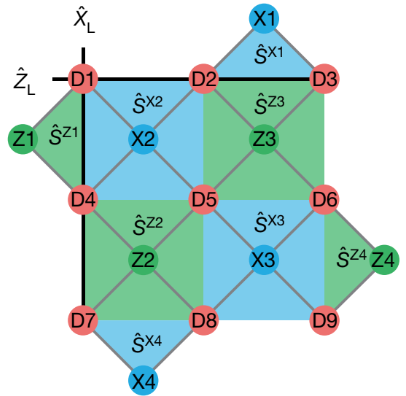
\includegraphics[width=0.2\textwidth]{sections/5_practical_implementation/representation.png}
    \caption{}
\end{figure}

\subsection{Realizing repeated quantum error correction in a distance-three surface code}
Successful implementation of the surface code is a milestone in quantum error correction, showing that practical realization is possible, we are one step closer to making a large-scale quantum computer. Using 17 physical qubits in a superconducting circuit, researchers have encoded quantum information in a distance-three logical qubit. In a correction cycle of 1.1 $(\mu s)$ that can correct both bit-flip and phase-flip errors, they have successfully preserved the cardinal states of the qubit. By repeatedly correcting errors, a low error rate of 3\% per cycle shows that the surface code does suppress the error probability as theory suggests. This breakthrough brings us closer to large quantum computing systems that can perform computation out of reach of the capacities of modern classical computers.

This achievement demonstrates the robustness of the surface code in a practical setup, supporting its potential for fault-tolerant quantum computing. By achieving low error rates and preserving qubit states, the experiment validates theoretical predictions and advances the development of scalable quantum computers.

\subsection{Repeated quantum error detection in a surface code}

The paper discusses the implementation of a minimal surface code for QEC using superconducting qubits. The surface code is a promising architecture for fault-tolerant quantum computing due to its high error threshold. In this study, the authors use seven superconducting qubits—four data qubits and three ancilla qubits—to repeatedly detect and correct any single error. This is a crucial step towards practical QEC, which is necessary for the realization of reliable and scalable quantum computers.

\begin{figure}[h]
    \centering
    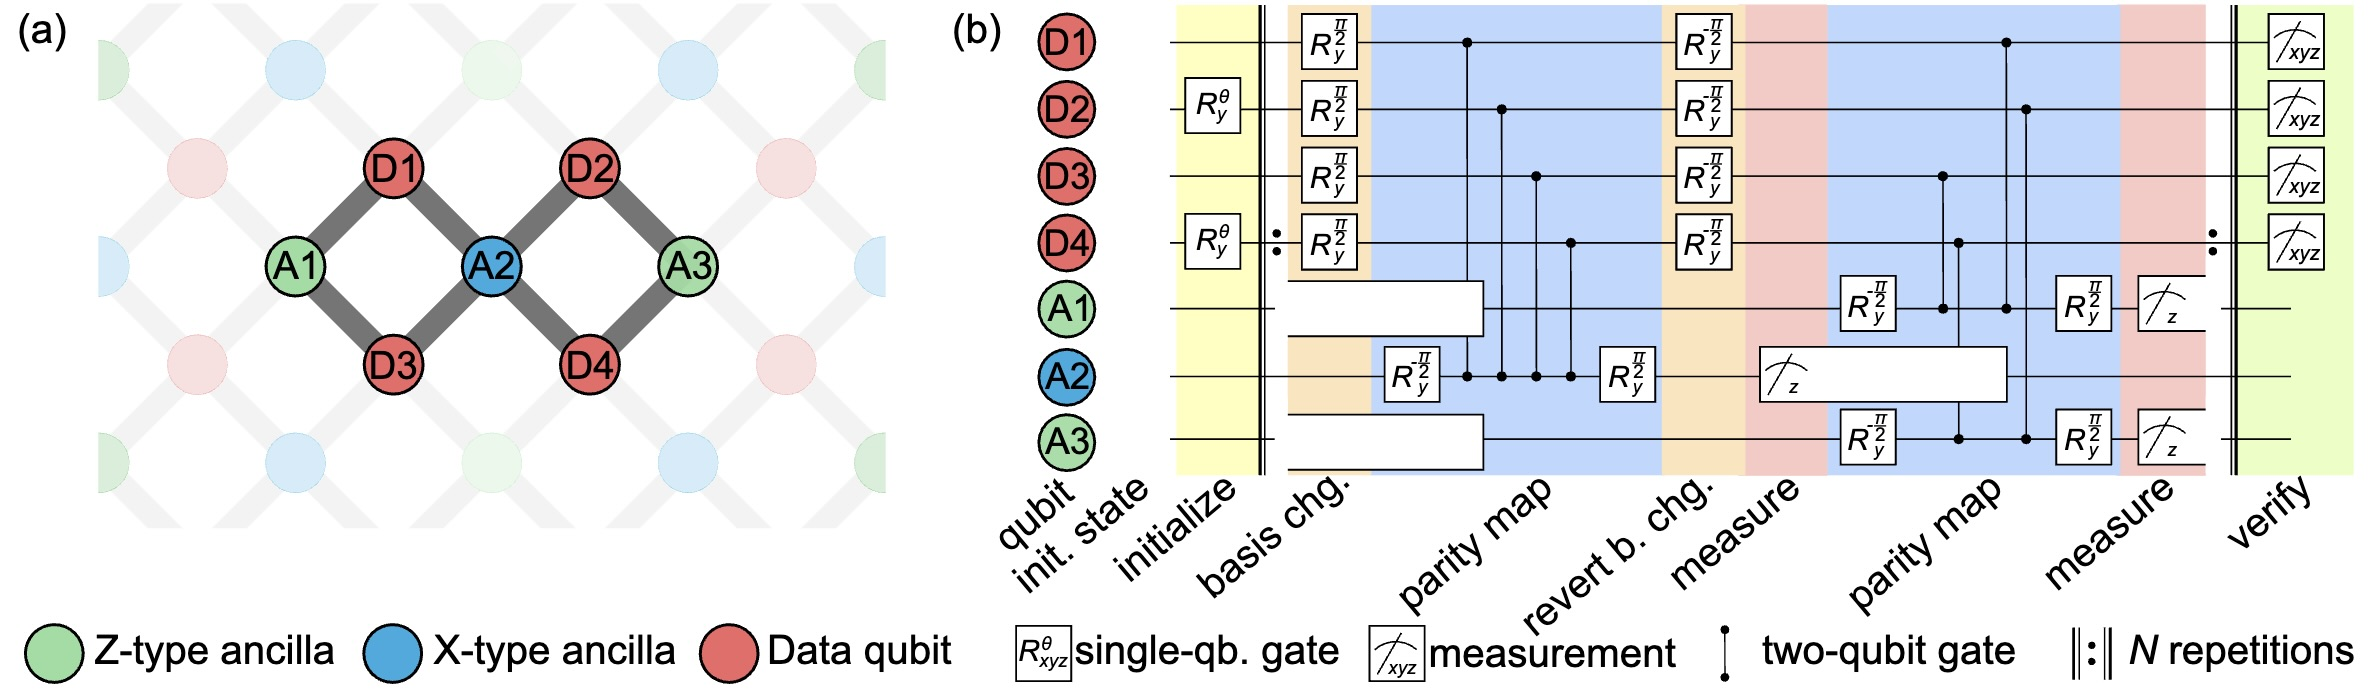
\includegraphics[width=0.4\textwidth]{sections/5_practical_implementation/7_qubits.jpg}
    \caption{}
\end{figure}

\begin{table}[h]
    \centering
    \caption{Lifetime/Coherence Time Comparison}
    \begin{center}
        \begin{tabular}{|c|c|c|}
            \hline
            \textbf{Error} & \textbf{Lifetime ($\mu s$)} & \textbf{Coherence Time ($\mu s$)} \\
            \hline
            Logical        & 62.5 ± 9.4                & 72.5 ± 32.9 \\
            Physical       & 16.8                      & 21.5        \\
            \hline
        \end{tabular}
    \end{center}
    \begin{tablenotes}
        \small
        \item \textbf{Note:} For both operators, the logical error probabilities per stabilizer measurement cycle are lower than the physical error rates of the qubits involved.
    \end{tablenotes}
\end{table}

Numerical simulations, accounting for factors like finite qubit lifetimes and coherence times, as well as residual $ZZ$ coupling and readout errors, show good agreement with the experimental data. The simulated logical decay times (44.2 ($\mu s$) for $Z_L$ and 59.6 ($\mu s$) for $X_L$) are within the experimental error bars.

\subsection{Low-distance surface codes under realistic quantum noise}

The paper investigates the practical implementation of distance-3 surface codes, which are a key component for scalable quantum computing. These surface codes are essential for achieving fault-tolerant quantum computation by correcting errors in quantum states. The authors focus on developing a circuit and a decoder tailored for the near-term experimental realization of these codes. They simulate the performance of the surface code under various realistic quantum noise models, such as amplitude and phase damping, and compare the results to those obtained using a Pauli-twirl approximation, finding that the approximation tends to provide a pessimistic threshold estimate.

As the figure~\ref{fig:25_qubits} below, the study delves into three specific types of surface code layouts: the standard 25-qubit layout, and two optimized layouts with 17 and 13 qubits, respectively. Each layout has distinct configurations and resource requirements, with the 17- and 13-qubit versions designed to reduce the number of physical qubits while maintaining error correction capabilities. The paper also details the construction of a fast decoder that operates in limited-memory, low-temperature environments, crucial for practical deployment.
\begin{figure}[h]
    \centering
    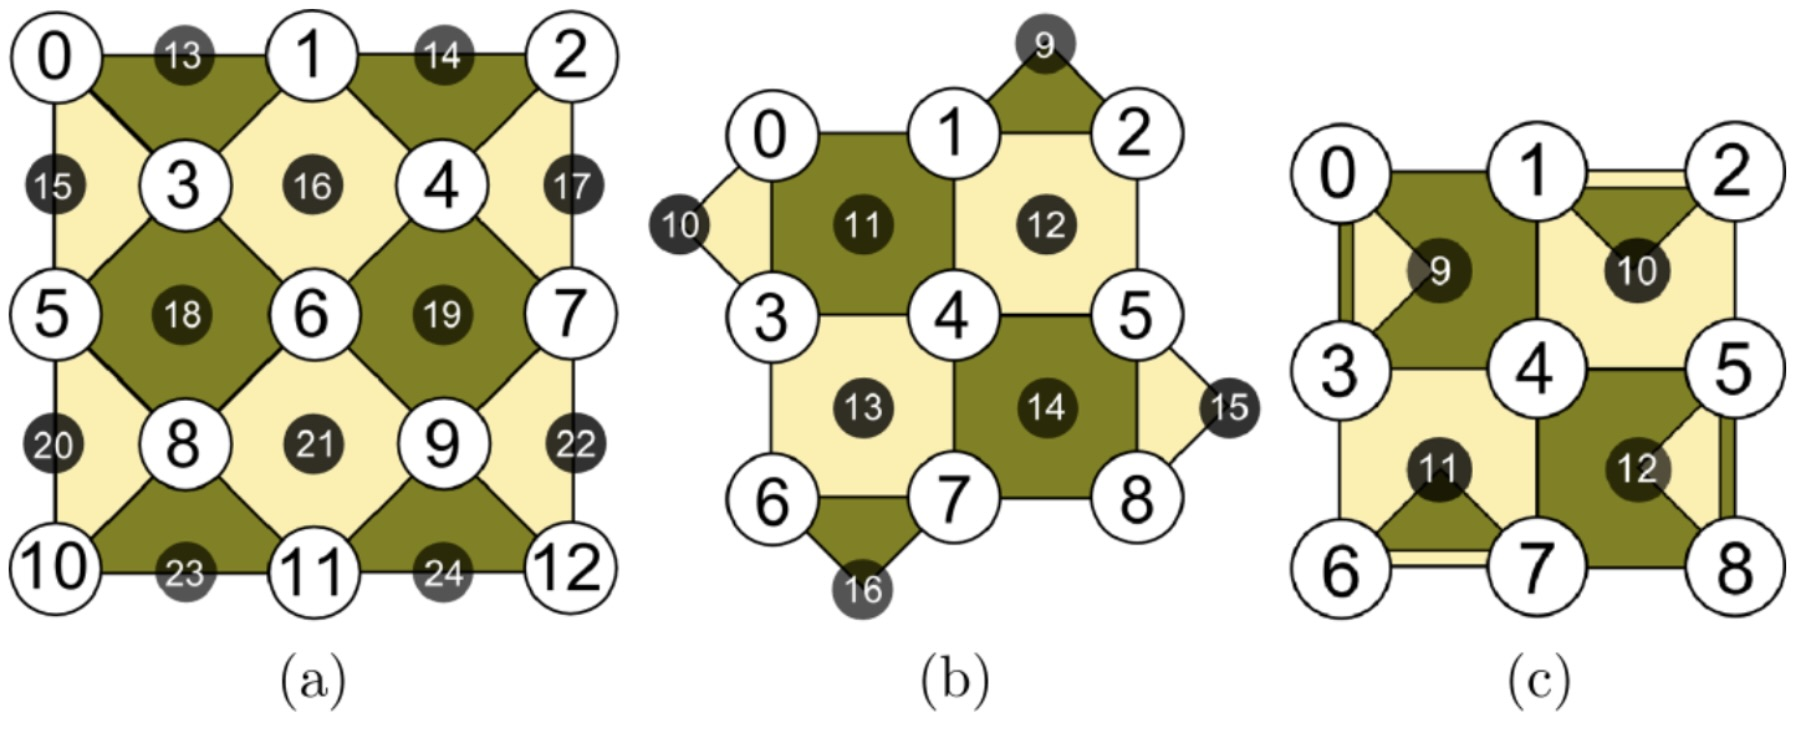
\includegraphics[width=0.3\textwidth]{sections/5_practical_implementation/25_qubits.jpg}
    \caption{(a) 25,(b) 17, and (c) 13 qubits. White circles represent data qubits, and black circles represent syndrome qubits. Dark square and triangular patches represent $X$ stabilizers; light patches represent $Z$ stabilizers. The layered patches on surface-13 indicate use of the syndrome qubit first to measure a four-qubit stabilizer and then to measure a two-qubit stabilizer.}
    \label{fig:25_qubits}
\end{figure}

In their simulations, the authors consider five types of flips that can occur in the quantum bits (qubits): bit flips, phase flips, and combinations of these errors. The simulations employ realistic noise models to determine the necessary gate and measurement speeds for achieving reliable error correction. For superconducting devices, they demonstrate that a qubit encoded in a 17-qubit surface code exhibits a significantly lower error rate compared to an unencoded qubit, provided the gate times range from 5 to 40 $(ns)$ and $T_1$ times (relaxation times) are at least 1 to 2 $(\mu s)$. In the context of ion trap devices, they find that gate times of 1 microsecond and $T_1$ times of at least 40 $(ms)$ are adequate to observe measurable differences in error rates.

\begin{figure}[h]
    \centering
    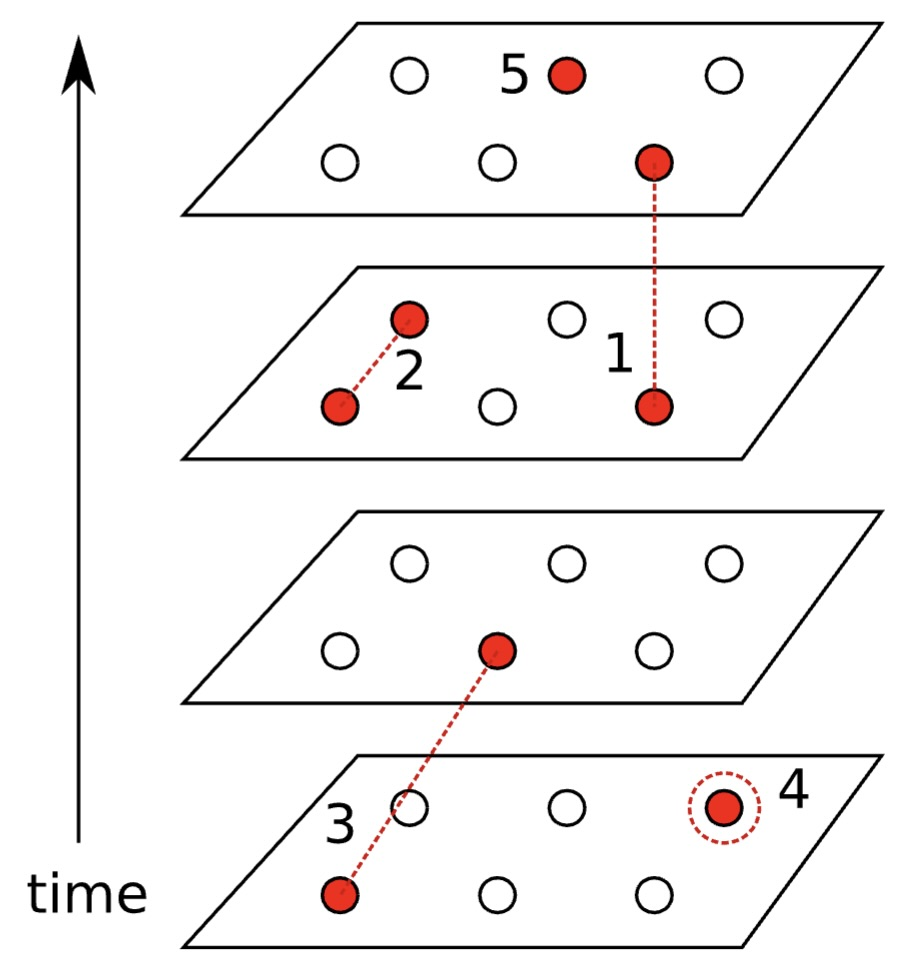
\includegraphics[width=0.2\textwidth]{sections/5_practical_implementation/LUT_rule.jpg}
    \caption{Lookup table decoding rules. Each circle represents a syndrome measurement. Filled (red) circles indicate "flips." Five types of flips are shown: (1) measurement error, (2,3) paired flips indicating a single-qubit error on the data qubit, (4) a single flip indicating one data-qubit error, and (5) and undetermined flip.}
    \label{fig:LUT_rule}
\end{figure}

The paper emphasizes the importance of these findings for the experimental demonstration and verification of small surface codes acting as single-qubit quantum memory. By presenting a framework for near-term implementation, the research paves the way for significant advancements in the field of quantum error correction and the development of robust quantum computing technologies.